\documentclass[main]{subfiles}

\begin{document}
\subsection{Modul To}
Efter at have målt switchen, som beskrevet i \cref{dataopsamling2}, konkluderes det, at system er hurtig nok til at måle et signal. Herefter måles laserstrålens waist, ved at logge den transmitterede intensitet som funktion af millimeterskrue. Dette ses på \cref{fig:graf3}.
\begin{figure}[H]
    \centering
    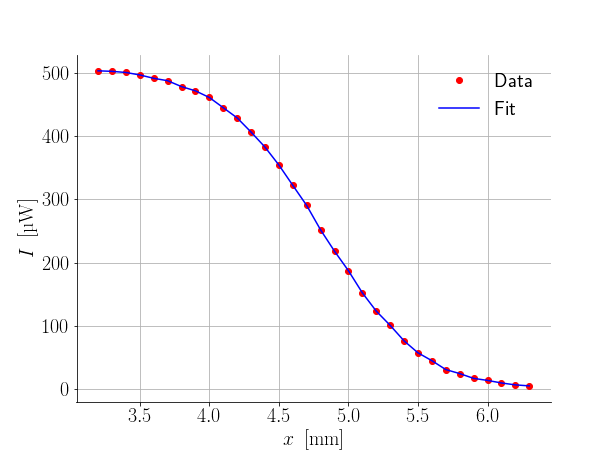
\includegraphics[width=\linewidth]{tegninger/graf3.png}
    \caption{}
    \label{fig:graf3}
\end{figure}
På \cref{fig:graf3} ses det at intensiteten af strålen falder mest når kniven er omkring midten af strålen, hvilket giver god mening idet at vi forventer at strålen fordeler sig omkring sin akse og vi dermed rammer mere af strålen omkring centrum. Umiddelbart ser figuren symmetrisk ud på den måde at den bevæger sig ensartet i bunden af grafen og toppen af grafen, hvilket understøtter forventningen om at strålen fordeler sig ensartet omkring laserens akse.
Ud fra figuren her kan waist, $w_0$ findes ved at indsætte nogle hjælpelinjer, netop da waist vil være forskellen i længde mellem de to punkter hvor intensiteten er 84\% og 16\% af max intensiteten.
\begin{figure}
  \centering
  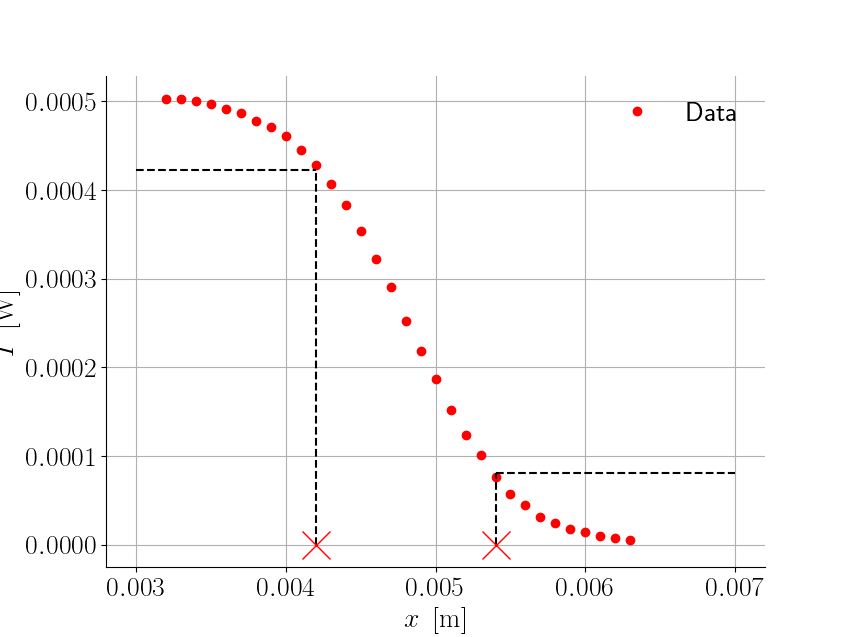
\includegraphics[width=\linewidth]{tegninger/graf_find_w.png.png}
  \caption{}
  \label{fig:graf_find_w}
\end{figure}
På \cref{fig:graf_find_w} ses de omtalte linjer og to røde krydser. De røde krydser indikerer punkterne hvor intensiteten er 84\% og 16\%. Det findes ud fra dette at afstanden mellem de to kryder bliver, $w_0 = 1,2 \pm 0,1 \ \si{\milli\meter}$. Usikkerheden her er netop usikkerheden på længdemålingerne, som grundet millimeterskruen er $0,1 \si{\milli\meter}$.



\end{document}
